\documentclass[11pt]{scrartcl}
\usepackage[T1]{fontenc}
\usepackage[utf8]{inputenc}

\title{Computer Systems Week 2 Lab}
\author{Daniel Coady (102084174)}
\date{07/08/2019}

\usepackage{graphicx}
\usepackage[colorlinks]{hyperref}
\usepackage{tgadventor}

\begin{document}

\sffamily

\maketitle

% 4-bit binary adder
\begin{center}
    \begin{tabular}{c c|c}
        \multicolumn{3}{c}{4-Bit Binary Adder} \\
        \hline
        input0 & input1 & output \\
        0101 & 0000 & 00101 \\
        0101 & 0001 & 00110 \\
        0101 & 0010 & 00111 \\
        0101 & 0011 & 01000 \\
        0101 & 0100 & 01001 \\
        0101 & 0101 & 01010 \\
        0101 & 0110 & 01011 \\
        0101 & 0111 & 01100 \\
        0101 & 1000 & 01101 \\
        0101 & 1001 & 01110 \\
        0101 & 1010 & 01111 \\
        0101 & 1011 & 10000 \\
        0101 & 1100 & 10001 \\
        0101 & 1101 & 10010 \\
        0101 & 1110 & 10011 \\
        0101 & 1111 & 10100 \\
    \end{tabular}

    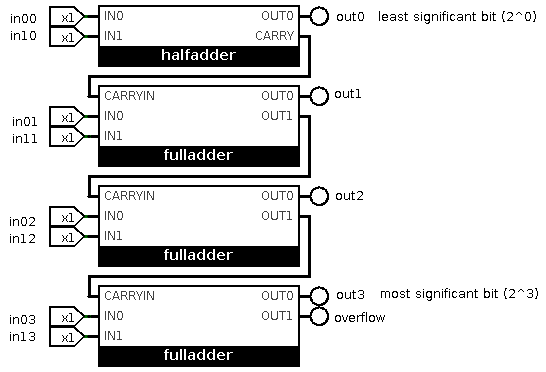
\includegraphics[scale=0.5]{images/4bitadder.png}
\end{center}

\pagebreak

% rs flip flop
\begin{center}
    \begin{tabular}{c c|c c}
        \multicolumn{4}{c}{RS Flip Flop} \\
        \hline
        set & reset & Qa & Qb \\
        1 & 0 & 0 & 1 \\
        1 & 1 & 0 & 0 \\
        0 & 1 & 1 & 0 \\
        1 & 1 & 0 & 0 \\
    \end{tabular}

    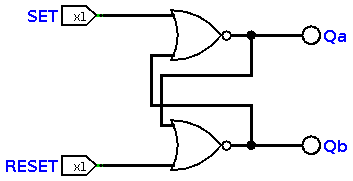
\includegraphics[scale=0.6]{images/rsflipflop.png}
\end{center}

When both inputs are on then both outputs turn off, which in a flip flop is an invalid state since Qb should always be the inverse of Qa.
The reason why this is an issue is because if we go from a state where both inputs are on to one where both are off, in the physical
realm we cannot predict what it's output would be since it would ultimately depend on which one is off first.

% d flip flop
\begin{center}
    \begin{tabular}{c c|c c}
        \multicolumn{4}{c}{D Flip Flop} \\
        \hline
        clk & set & Qa & Qb \\
        0 & 0 & 0 & 1 \\
        0 & 1 & 0 & 1 \\
        1 & 1 & 1 & 0 \\
        1 & 0 & 0 & 1 \\
    \end{tabular}

    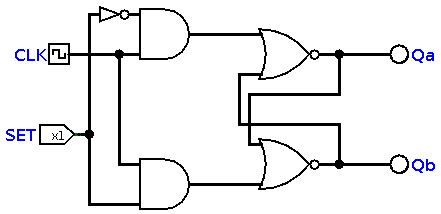
\includegraphics[scale=0.6]{images/dflipflop.png}
\end{center}

The D Flip Flop works by matching the set input when the clock input is on. This allows us to synchronize it to a circuit's clock which is
useful in circuit design for time sensitive tasks where you need to be sure that certain actions are synchroized with each other. This is
used over the RS Flip Flop because it is both synchronized to a clock as well as completely safe to indeterminite states, or in other
words the output is always predictable.

% jk flip flop
\begin{center}
    \begin{tabular}{c c|c c}
        \multicolumn{4}{c}{JK Flip Flop} \\
        \hline
        J & K & Qa & Qb \\
        0 & 0 & 0 & 1 \\
        1 & 0 & 1 & 0 \\
        0 & 1 & 0 & 1 \\
        1 & 1 & 1 & 0 \\
    \end{tabular}

    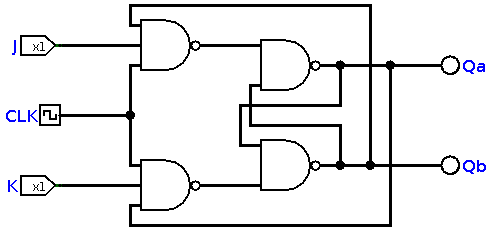
\includegraphics[scale=0.6]{images/jkflipflop.png}
\end{center}

The reason why the JK Flip Flop is considered a more programmable and general purpose flip flop is because of how you can adapt it's use to
a D or T Flip Flop. To make it work like a D Flip Flop you simply control it with the J and K inputs to make Qa on or off respectively
on a clock cycle. To make it work like a T Flip Flop then all you need to do is turn both J and K inputs on, which will in turn toggle Qa
on and off with each clock cycle.

\end{document}
